%%%%%%%%%%%%%%%%%%%%%%%%%%%%%%%%%%%%%%%%%
% Beamer Presentation
% LaTeX Template
% Version 1.0 (10/11/12)
%
% This template has been downloaded from:
% http://www.LaTeXTemplates.com
%
% License:
% CC BY-NC-SA 3.0 (http://creativecommons.org/licenses/by-nc-sa/3.0/)
%
%%%%%%%%%%%%%%%%%%%%%%%%%%%%%%%%%%%%%%%%%

%----------------------------------------------------------------------------------------
%	PACKAGES AND THEMES
%----------------------------------------------------------------------------------------

\documentclass[french]{beamer}
\usepackage[french]{babel}
\usepackage[T1]{fontenc}
\usepackage{lmodern}
\usepackage[utf8]{inputenc}

\newcommand{\handout}[5]{
  \noindent
  \begin{center}
  \framebox{ \vbox{ \hbox to 5.78in { {\bf IFT2125 -- Introduction à
          l'algorithmique } \hfill #2 }
      \vspace{4mm}
      \hbox to 5.78in { {\Large \hfill #5  \hfill} }
      \vspace{2mm}
      \hbox to 5.78in { {\hfill \em #3 \hfill} }
    }
  }
  \end{center}
  \vspace*{4mm}
}
\mode<presentation> {

% The Beamer class comes with a number of default slide themes
% which change the colors and layouts of slides. Below this is a list
% of all the themes, uncomment each in turn to see what they look like.

%\usetheme{default}
%\usetheme{AnnArbor}
%\usetheme{Antibes}
%\usetheme{Bergen}
%\usetheme{Berkeley}
%\usetheme{Berlin}
%\usetheme{Boadilla}
%\usetheme{CambridgeUS}
%\usetheme{Copenhagen}
%\usetheme{Darmstadt}
%\usetheme{Dresden}
%\usetheme{Frankfurt}
%\usetheme{Goettingen}
%\usetheme{Hannover}
%\usetheme{Ilmenau}
%\usetheme{JuanLesPins}
%\usetheme{Luebeck}
\usetheme{Madrid}
%\usetheme{Malmoe}
%\usetheme{Marburg}
%\usetheme{Montpellier}
%\usetheme{PaloAlto}
%\usetheme{Pittsburgh}
%\usetheme{Rochester}
%\usetheme{Singapore}
%\usetheme{Szeged}
%\usetheme{Warsaw}

% As well as themes, the Beamer class has a number of color themes
% for any slide theme. Uncomment each of these in turn to see how it
% changes the colors of your current slide theme.

%\usecolortheme{albatross}
%\usecolortheme{beaver}
%\usecolortheme{beetle}
%\usecolortheme{crane}
%\usecolortheme{dolphin}
%\usecolortheme{dove}
%\usecolortheme{fly}
%\usecolortheme{lily}
%\usecolortheme{orchid}
%\usecolortheme{rose}
%\usecolortheme{seagull}
%\usecolortheme{seahorse}
%\usecolortheme{whale}
%\usecolortheme{wolverine}

%\setbeamertemplate{footline} % To remove the footer line in all slides uncomment this line
\setbeamertemplate{footline}[page number] % To replace the footer line in all slides with a simple slide count uncomment this line

\setbeamertemplate{navigation symbols}{} % To remove the navigation symbols from the bottom of all slides uncomment this line
}

\usepackage{graphicx} % Allows including images
\usepackage{booktabs} % Allows the use of \toprule, \midrule and \bottomrule in tables

%----------------------------------------------------------------------------------------
%	TITLE PAGE
%----------------------------------------------------------------------------------------

\title[Intro-ML]{Briève introduction à l'apprentissage machine} % The short title appears at the bottom of every slide, the full title is only on the title page

\author{Nicolas Hurtubise \\
Vincent Antaki} % Your name
\institute[UdeM] % Your institution as it will appear on the bottom of every slide, may be shorthand to save space
{
*Ou introduction aux modèles d'apprentissages non-paramétrés \\ % Your institution for the title page
\medskip
\textit{hurtubin@iro.umontreal.ca
\\antakivi@iro.umontreal.ca} % Your email address
}
\date{} % Date, can be changed to a custom date

\begin{document}

\begin{frame}
\titlepage % Print the title page as the first slide
\end{frame}


%----------------------------------------------------------------------------------------
%	PRESENTATION SLIDES
%----------------------------------------------------------------------------------------

%------------------------------------------------
\begin{frame}
\frametitle{L'apprentissage machine ?}

Selon \textbf{\href{http://www.iro.umontreal.ca/~aimeur/cours/ift6261/Survol_apprentissage_machine.pdf}{Sébastien
Gambs}}

\begin{quote}
L'apprentissage machine étudie les techniques permettant de donner à la machine la capacitée d'apprendre à partir d'expériences passées
\end{quote}
\begin{center}\rule{3in}{0.4pt}\end{center}
\end{frame}

\begin{frame}
\frametitle{Quel rapport avec l'UdeM ?}

\begin{itemize}
\item Pionnière de la technique des réseaux profonds (le modèle trendy en ce moment) avec l'Université de Toronto et l'Université de New York.
\item Un pas mal gros laboratoire d'apprentissage-machine.
\end{itemize}

\begin{center}\rule{3in}{0.4pt}\end{center}

\end{frame}


\begin{frame}
\frametitle{Grosso-modo c'est quoi?}

\begin{quote}
Champ d'étude de l'intelligence artificielle visant à apprendre à partir d'exemples les paramètres d'un modèle en vue d'accomplir une tâche.
\end{quote}
\end{frame}

\begin{frame}
\frametitle{Un modèle?}
\begin{itemize}
\item Le modèle est la partie la plus importante de tout algorithme d'apprentissage. Un modèle définit une fonction de décision et, du coup, les paramètres à apprendre.

\item Ex. : Une ligne peut servir à classifier un ensemble en 2 sections. 

	$$f(x): ax + b$$

Par exemple, nous avons la position et l'équipe des joueurs sur un terrain de ballon-chasseur. Nous cherchons à estimer la position de la ligne du milieu du terrain en fonction des joueurs.
\begin{center}
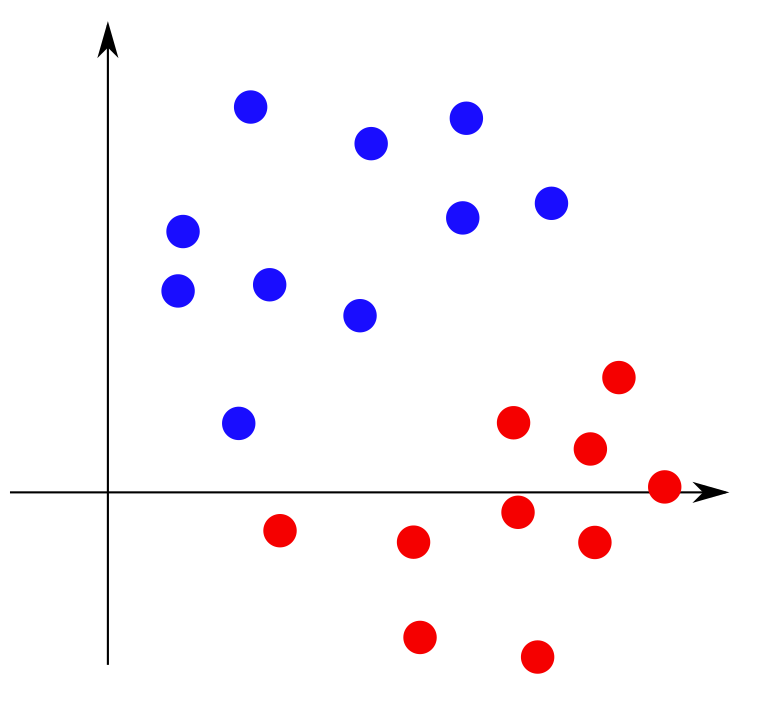
\includegraphics[scale=0.2]{ballon-chasseur.png}
\end{center}

\end{itemize}

\end{frame}

\begin{frame}
\frametitle{Les hyper-paramètres}

\begin{itemize}
\item La capacité d'un modèle est déterminée par sa configuration (que l'on nomme hyper-paramètres)

\item Ex. Un polynôme de degré $k$ à la place d'une ligne.
\end{itemize}

\begin{tabular}{ccc}
Degré (hyper-p.) & Fonction de décision & Paramètres à apprendre \\
$0$	& $f(x) = a$ & $a$ \\
$1$ & $f(x) = ax+b$ & $a,b$ \\
$2$ & $f(x) = ax^2 + bx + c$ & $a,b,c$ \\
etc..& &
\end{tabular}

\end{frame}



\begin{frame}[fragile]
\frametitle{Problème général : classifier une donnée selon ses
caractéristiques}

\begin{center}
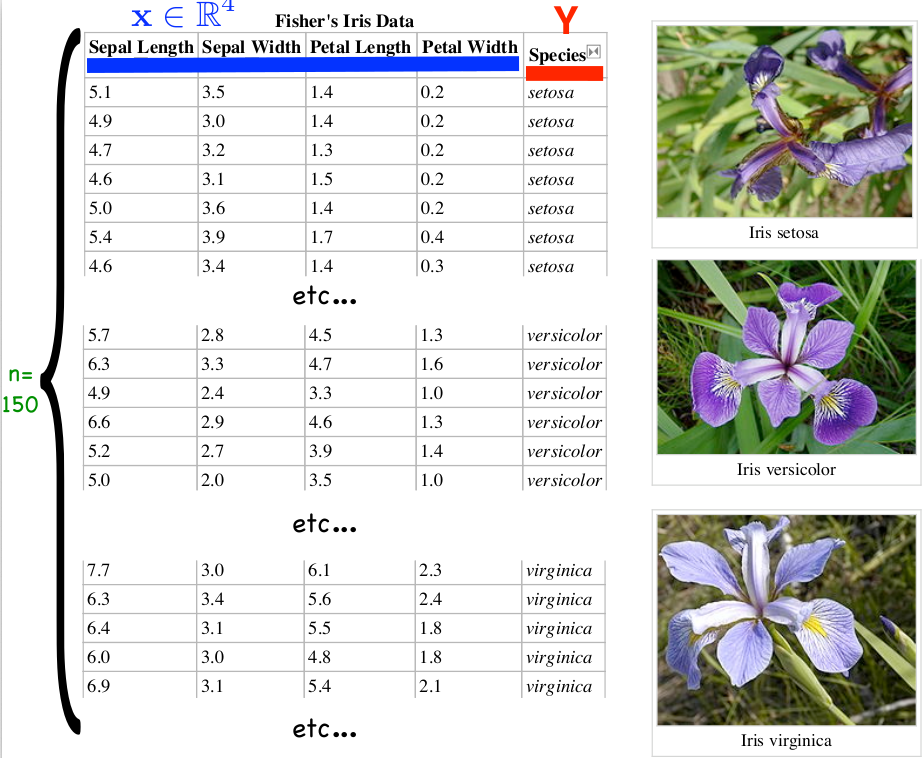
\includegraphics[scale=0.25]{10.png}
\end{center}

\end{frame}

\begin{frame}[fragile]
\frametitle{Classifier une donnée selon ses
caractéristiques}

\begin{center}
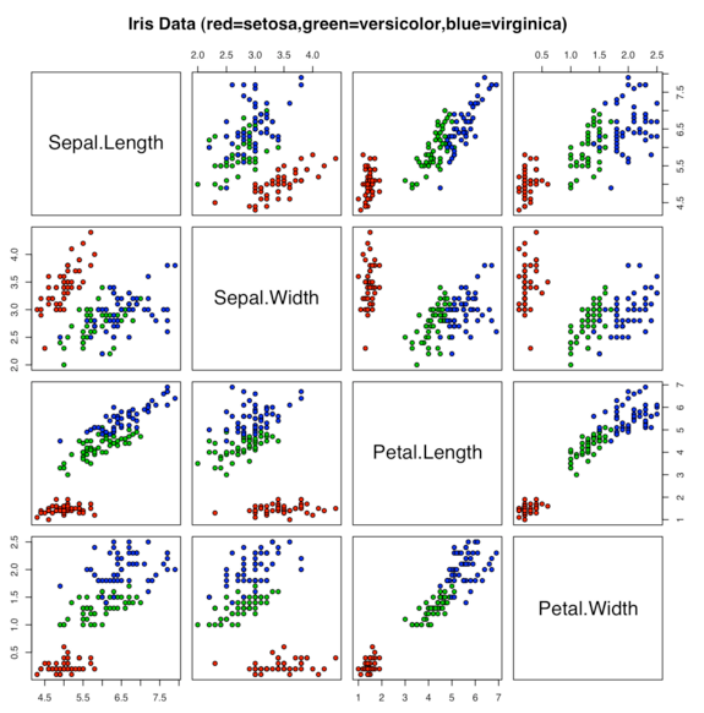
\includegraphics[scale=0.3]{11.png}
\end{center}

\end{frame}



\begin{frame}
\frametitle{Qu'est-ce qu'on fait ici?}

\begin{itemize}
\item Nous allons vous montrer deux techniques de modèle non-paramétrés (non-paramétrés : les techniques n'apprennent pas à proprement parler de paramètres, elles ne font que garder en mémoire tous les exemples et calculent une réponse directement en fonction de ceux-ci)
\item Nous allons ici tenter de classifier des couleurs en fonction de millions de données récoltés par sondage internet. 
\end{itemize}

\end{frame}


\begin{frame}[fragile]
\frametitle{Problème : Apprendre à nommer des
couleurs}

On cherche un algorithme qui peut nous donner le nom d'une couleur selon
sa valeur \texttt{rgb}

{Exemples}

\begin{verbatim}
    rgb(255, 0, 0) -> Rouge
    rgb(0, 255, 0) -> Vert
    rgb(0, 0, 255) -> Bleu
    rgb(0, 0, 0) -> Noir
    rgb(255, 255, 255) -> Blanc
    rgb(200, 80, 180) -> ?
\end{verbatim}

\begin{center}\rule{3in}{0.4pt}\end{center}
\end{frame}

\begin{frame}
\frametitle{Données : xkcd's color dataset}

\begin{itemize}
\item L'auteur du webcomic XKCD a récolté plus de 3 millions d'échantillons de couleur étiquetée par des utilisateurs du web

\item Comme on peut s'y attendre, une certaine proportion des données est aberrante (lire *troll*).

\item Chaque exemple est stocké sous forme de paires (rgb, étiquettes).
\end{itemize}

\end{frame}


\begin{frame}[fragile]
\frametitle{Approche : Séparer en sections et trouver la tendance}

Technique de l'histogramme :
\begin{itemize}
\item Prendre l'espace d'entrée et le découper en sections de taille équivalente. 

\begin{center}
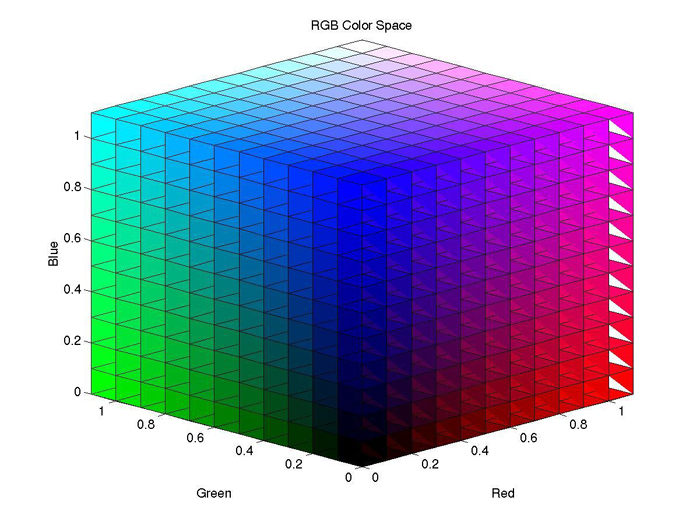
\includegraphics[scale=0.25]{RGB-color-space.jpg}
\end{center}
		
\item Calculer la classe majoritaire des exemples dans chaque section et assigner sa valeur à la section.


\end{itemize}

\end{frame}

\begin{frame}
\frametitle{Approche : Séparer en sections et trouver la tendance}

{Avantages}

\begin{itemize}
\itemsep1pt\parskip0pt\parsep0pt
\item
  Très simple, semble suffisant dans certains cas.
\end{itemize}

{Problèmes}

\begin{itemize}
\itemsep1pt\parskip0pt\parsep0pt
\item
  Certaines catégories peuvent être vides

  \begin{itemize}
  \itemsep1pt\parskip0pt\parsep0pt
  \item
    Impossible de donner une réponse dans certains cas
  \end{itemize}
\item
  Il faut trouver le nombre idéal de catégories

  \begin{itemize}
  \itemsep1pt\parskip0pt\parsep0pt
  \item
    Pas assez de catégories ne donne pas une idée assez précise
  \item
    Trop de catégories risque de donner beaucoup de cas où on ne sait
    pas répondre
  \end{itemize}
  \item La méthode est complètement inadaptée pour certaines tâches.
  \begin{itemize}
	\item La prochaine méthode est beaucoup plus versatile et généralement plus efficace.  
  
  \end{itemize}  	
	
\end{itemize}
\end{frame}

\begin{frame}
\frametitle{Autre approche : Les $k$ plus proches voisins}
Trouver les $k$ éléments les plus "proches" à ce qu'on cherche à identifier et déduire une catégorie en fonction de ces éléments (et potentiellement de leur distance)
\begin{center}
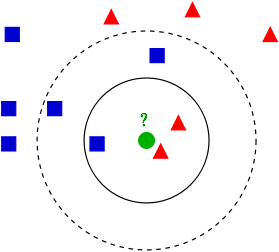
\includegraphics[scale=0.4]{KnnClassification.png}
\end{center}

Les voisins : $((x_1,y_1),(x_2,y_2),...,(x_k,y_k))$ (x la position, y la couleur)
\end{frame}

\begin{frame}
\frametitle{Autre approche : Les $k$ plus proches voisins}

\begin{itemize}

\item{Nécessite une définition de la distance entre 2 couleurs (distance euclidienne en 3 dimension dans notre cas)}

Pour $a$ et $b$, deux tableaux de nombre de taille 3, la distance se définit comme suit :
$$ d(a,b) = \sqrt{(a_1-b_1)^2+(a_2-b_2)^2+(a_3-b_3)^2}$$

\item{Nécessite une fonction de score. La catégorie choisie sera celle avec le plus haut score.}
\end{itemize}

\end{frame}

\begin{frame}
\frametitle{Fonctions de scores}
Plusieurs variantes existent :
\begin{itemize}
\item{Vote majoritaire des k plus proches voisins}\\
Score(Couleur) = Compte des couleurs de cette catégorie

\item{Vote pondéré de tous les points dans l'ensemble}\\

Score(Couleur, position) = Sommes de $\frac{1}{dist(x_i,p)}$ pour tous les $x_i$ tel que $y_i$ est la couleur demandée

$$\text{score}(c, p) = \sum_{i=1}^k I_{c=y_i} \cdot \frac{1}{d_(x_i,p)}$$
\item{Vote pondéré des k plus proches voisins}\\


\item{Votre propre variante}\\

\end{itemize}

\end{frame}

\begin{frame}
\frametitle{Exemple de résultats}
\begin{itemize}
\item 1 plus proche voisin, vote majoritaire :
\begin{center}
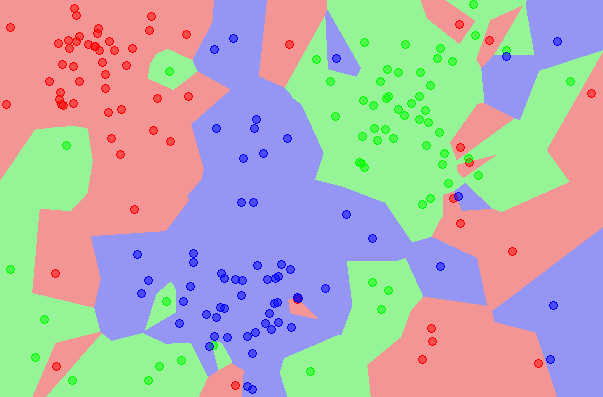
\includegraphics[scale=0.3]{Map1NN.png}
\end{center}

\item 5 plus proches voisins, vote majoritaire :
\begin{center}
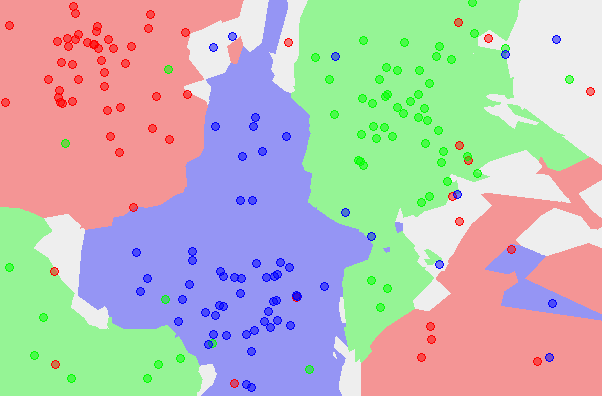
\includegraphics[scale=0.3]{Map5NN.png}
\end{center}
\end{itemize}

\end{frame}



\begin{frame}
\frametitle{Contrôle de la capacité}
Vous vous rappelez des hyper-paramètres? Ceux-ci contrôlent la capacité des modèles à apprendre. 

\begin{itemize}
\item Histogramme : le nombre de séparations dans chaque dimension
\item KNN : le nombre de voisins
\end{itemize}

Mal ajustés, ils peuvent causer des réponses erronées et des aberations. Trop apprendre peut être aussi dommageable que pas assez.
\end{frame}

\begin{frame}
\frametitle{Questions}

\begin{center}
Des questions?
\end{center}

\end{frame}

\end{document}
